\documentclass[journal]{vgtc}                     % final (journal style)
%\documentclass[journal,hideappendix]{vgtc}        % final (journal style) without appendices
%\documentclass[review,journal]{vgtc}              % review (journal style)
%\documentclass[review,journal,hideappendix]{vgtc} % review (journal style)
%\documentclass[widereview]{vgtc}                  % wide-spaced review
%\documentclass[preprint,journal]{vgtc}            % preprint (journal style)


%% Uncomment one of the lines above depending on where your paper is
%% in the conference process. ``review'' and ``widereview'' are for review
%% submission, ``preprint'' is for pre-publication in an open access repository,
%% and the final version doesn't use a specific qualifier.

%% If you are submitting a paper to a conference for review with a double
%% blind reviewing process, please use one of the ``review'' options and replace the value ``0'' below with your
%% OnlineID. Otherwise, you may safely leave it at ``0''.
\onlineid{0}

%% In preprint mode you may define your own headline. If not, the default IEEE copyright message will appear in preprint mode.
%\preprinttext{To appear in IEEE Transactions on Visualization and Computer Graphics.}

%% In preprint mode, this adds a link to the version of the paper on IEEEXplore
%% Uncomment this line when you produce a preprint version of the article 
%% after the article receives a DOI for the paper from IEEE
%\ieeedoi{xx.xxxx/TVCG.201x.xxxxxxx}

%% declare the category of your paper, only shown in review mode
\vgtccategory{Research}

%% please declare the paper type of your paper to help reviewers, only shown in review mode
%% choices:
%% * algorithm/technique
%% * application/design study
%% * evaluation
%% * system
%% * theory/model
\vgtcpapertype{please specify}

%% Paper title.
\title{Global Illumination for Fun and Profit}

%% Author ORCID IDs should be specified using \authororcid like below inside
%% of the \author command. ORCID IDs can be registered at https://orcid.org/.
%% Include only the 16-digit dashed ID.
\author{%
  \authororcid{Josiah S.\ Carberry}{0000-0002-1825-0097},
  Ed Grimley, and 
  Martha Stewart
}

\authorfooter{
  %% insert punctuation at end of each item
  \item
  	Josiah Carberry is with Brown University.
  	E-mail: jcarberry@example.com
  \item
  	Ed Grimley is with Grimley Widgets, Inc.
  	E-mail: ed.grimley@example.com.

  \item Martha Stewart is with Martha Stewart Enterprises at Microsoft
  Research.
  	E-mail: martha.stewart@example.com.
}

%% Abstract section.
\abstract{%
  \lipsum[1] % filler text. Replace with your abstract.
  %
  %% We recommend that you link to your supplemental material here in the abstract, as well
  %% as in the Supplemental Materials section at the end.
  A free copy of this paper and all supplemental materials are available at \url{https://OSF.IO/2NBSG}.
}

%% Keywords that describe your work. Will show as 'Index Terms' in journal
%% please capitalize first letter and insert punctuation after last keyword
\keywords{Radiosity, global illumination, constant time}

%% A teaser figure can be included as follows
\teaser{
  \centering
  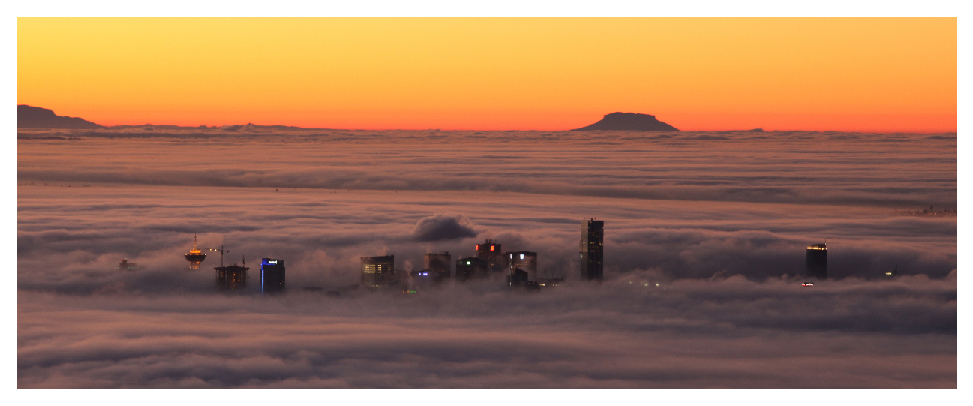
\includegraphics[width=\linewidth, alt={A view of a city with buildings peeking out of the clouds.}]{CypressView}
  \caption{%
  	In the Clouds: Vancouver from Cypress Mountain.
  	Note that the teaser may not be wider than the abstract block.%
  }
  \label{fig:teaser}
}

%% Uncomment below to disable the manuscript note
%\renewcommand{\manuscriptnotetxt}{}

%% Copyright space is enabled by default as required by guidelines.
%% It is disabled by the 'review' option or via the following command:
%\nocopyrightspace


%%%%%%%%%%%%%%%%%%%%%%%%%%%%%%%%%%%%%%%%%%%%%%%%%%%%%%%%%%%%%%%%
%%%%%%%%%%%%%%%%%%%%%% LOAD PACKAGES %%%%%%%%%%%%%%%%%%%%%%%%%%%
%%%%%%%%%%%%%%%%%%%%%%%%%%%%%%%%%%%%%%%%%%%%%%%%%%%%%%%%%%%%%%%%

%% Tell graphicx where to find files for figures when calling \includegraphics.
%% Note that due to the \DeclareGraphicsExtensions{} call it is no longer necessary
%% to provide the the path and extension of a graphics file:
%% 
\includegraphics{diamondrule} is completely sufficient.
\graphicspath{{figs/}{figures/}{pictures/}{images/}{./}} % where to search for the images

%% Only used in the template examples. You can remove these lines.
\usepackage{tabu}                      % only used for the table example
\usepackage{booktabs}                  % only used for the table example
\usepackage{lipsum}                    % used to generate placeholder text
\usepackage{mwe}                       % used to generate placeholder figures

%% We encourage the use of mathptmx for consistent usage of times font
%% throughout the proceedings. However, if you encounter conflicts
%% with other math-related packages, you may want to disable it.
\usepackage{mathptmx}                  % use matching math font


\newcommand{\squishlist}{
 \begin{list}{$\bullet$}
 { \setlength{\itemsep}{0pt}
   \setlength{\parsep}{3pt}
   \setlength{\topsep}{3pt}
   \setlength{\partopsep}{0pt}
   \setlength{\leftmargin}{1.2em}
   \setlength{\labelwidth}{1em}
   \setlength{\labelsep}{0.6em}
 }
}
\newcommand{\squishend}{
 \end{list}
}



\newcommand{\stitle}[1]{\vspace*{0.4em}\noindent{\bf #1.\/}}
\newcommand{\sstitle}[1]{\vspace*{0.4em}\noindent{\bf #1:\/}}

\newcommand{\trim}{\vspace{-2mm}}
\newcommand{\ttrim}{\vspace{-1mm}}




\begin{document}

%%%%%%%%%%%%%%%%%%%%%%%%%%%%%%%%%%%%%%%%%%%%%%%%%%%%%%%%%%%%%%%%
%%%%%%%%%%%%%%%%%%%%%% START OF THE PAPER %%%%%%%%%%%%%%%%%%%%%%
%%%%%%%%%%%%%%%%%%%%%%%%%%%%%%%%%%%%%%%%%%%%%%%%%%%%%%%%%%%%%%%%

%% The ``\maketitle'' command must be the first command after the
%% ``\begin{document}'' command. It prepares and prints the title block.
%% the only exception to this rule is the \firstsection command
\firstsection{Introduction}

\maketitle

Tree-structured data are widely used to represent hierarchical information and model complex processes, such as organizational hierarchies, query plan trees in relational databases, reasoning trees in search and inference tasks, and abstract syntax trees (ASTs) in program analysis. In many real-world scenarios these trees are not static. They evolve over time or across steps as rules are applied, states are updated, search progresses, or human edits are introduced, forming sequences of tree transformations. Analyzing tree evolution is important for understanding how hierarchical structures change, identifying critical transition steps, and diagnosing abnormal or inefficient processes.

Compared with tree sequence analysis that treats trees primarily as a series of snapshots, Tree Evolution analysis focuses not only on what a tree looks like at a given step, but also with how one tree transforms into the next and why these changes occur. In many applications, the final tree only reflects the result of an evolving process, while obscuring key rewrites, backtracking behaviors, or local irregularities along the way. For example, in query optimization, an initial logical plan may go through a series of rule-based rewrites and structural adjustments before becoming an executable plan. Examining this process can help analysts understand optimizer behavior and locate the steps that lead to incorrect results or performance degradation. Similarly, in reasoning and search tasks, tree expansion, pruning, and rollback reveal the exploration strategy of the system; in program evolution analysis, local modifications on ASTs and their propagated effects can help expose refactoring behavior and error sources. These examples suggest that trees should often be understood as evolving structures rather than isolated snapshots.

Despite its importance, visual analytics of Tree Evolution remains challenging in at least three aspects. First, prior studies have shown that even comparing relatively simple graphs can be difficult for analysts~\cite{}, because topological comparison often disrupts cognitive continuity. This challenge becomes even greater in Tree Evolution analysis, where analysts must not only identify structural differences but also understand how one tree transforms into the next. Second, local topological changes are often scattered across large unchanged contexts, making it difficult to highlight critical differences without losing the structural context needed for interpretation. Third, critical changes in long evolution sequences are often sparse, making it hard to summarize major trends while preserving key transition steps. 

Existing studies have explored related problems from several perspectives, such as domain-specific evolution analysis, dynamic tree visualization, structural comparision, and temporal visual analytics. Some approaches are designed for specific application domains. For example, QOVIS~\cite{} supports the analysis of query
optimization process by leveraging domain knowledge. While such systems are effective in their target settings like the optimization rules. They rely on strong domain assumptions and are difficult to generalize to other tasks. Other approaches use animation~\cite{} or dynamic tree views~\cite{} to present transitions between adjacent steps, which can help reveal local continuity but become less effective for reviewing long sequences, locating critical steps, or comparing sparse changes across time. Temporal visual analytics methods can summarize trends and high-level stage-wise patterns, but they often ignore the topological structure and fine-grained change semantics of the trees. 
%Overall, existing approaches still fall short of jointly supporting topology-aware comparison between adjacent trees, context-preserving representation of critical differences, and long-sequence change summarization. 总觉得这里有点不到位，为什么需要我们的工作还是不够突出

%To address this gap, we propose \sysname{}, a topology-aware visual analytics framework for Tree Evolution. \sysname{} supports analysis at three levels. At the modeling level, it estimates corresponding changes between adjacent trees, representing evolution as a sequence of analyzable local change units rather than a set of disconnected snapshots. At the structural comparison level, it extracts compact difference-aware substructures that preserve essential context while reducing visual complexity, helping analysts focus on critical topological changes. At the sequence level, it organizes and simplifies local differences over time to reveal salient intervals, key transition steps, and overall evolutionary trends. By combining change modeling, topology-aware difference visualization, and sequence summarization, \sysname{} supports multi-granularity analysis from local changes to global evolution patterns.



%To address this gap, we propose \sysname{}, a topology-aware visual analytics framework for the evolution of tree structures. \sysname{} first computes topological differences between adjacent trees and identifies changed nodes, representing evolution as a sequence of local structural changes rather than disconnected snapshots. Based on these differences, it extracts and organizes difference-aware substructures that preserve essential context while reducing visual complexity, enabling effective comparison of topological differences without lose general context. \sysname{} further traces the lifecycle of nodes throughout the evolution process to support localized temporal analysis of changes. Building on these local analyses, it simplifies long sequences based on the distribution of differences to reveal salient intervals, key transition steps, and overall evolutionary trends. In this way, \sysname{} supports multi-granularity analysis from local changes to global evolution patterns.

To address this gap, we propose \sysname{}, a topology-aware visual analytics framework for the evolution of tree structures. \sysname{} first computes topological differences between adjacent trees and identifies changed nodes, representing the evolution as a sequence of local structural changes rather than a set of disconnected snapshots. It then extracts and organizes compact difference-aware substructures that preserve essential context while reducing visual complexity, enabling effective comparison of critical topological differences. Furthermore, \sysname{} traces the lifecycle of nodes throughout the evolution process to track the development of important information over time. Building on these local analyses, \sysname{} simplifies long sequences based on the distribution of differences to reveal salient intervals, key transition steps, and overall evolutionary trends. In this way, Building on these techniques, \sysname{} supports multi-granularity analysis from local changes to global evolution patterns.

The contributions of this work are as follows:

\squishlist
\item We formulate design requirements of \sysname, which addresses the core challenges of Tree Evolution as a visual analytics problem, including topology-aware comparison, context-preserving difference analysis, and long-sequence summarization.

%We formulate Tree Evolution as a visual analytics problem that jointly involves topology-aware comparison, context-preserving difference analysis, and long-sequence summarization, and we characterize common analytical needs shared across multiple application scenarios.

\item We propose a configurable differencing method for adjacent tree structures to estimate corresponding changes and evolution processes, and further develop a compact difference-aware substructure extraction strategy that balances fidelity and cognitive load.

\item We design and implement \sysname{}, a multi-granularity visual analytics framework that supports local topology comparison, cross-step evolution tracing, and long-sequence summarization of key processes.

\item We demonstrate the effectiveness and practical value of \sysname{} through multiple case studies and user interviews in tasks involving tree evolution understanding, key change localization, and long-sequence analysis.

\squishend

The remaining parts of the paper are organized as follows:


\section{Related Work}

\subsection{Dynamic Tree Visualization}

A substantial body of work has studied how to visualize hierarchical structures that evolve over time, with particular emphasis on preserving structural readability and supporting users' mental continuity across timesteps. One representative direction focuses on stable space-filling layouts for evolving hierarchies. Temporal Treemaps transforms a sequence of trees with known correspondences into a static nested treemap, allowing users to inspect appearance, disappearance, merge, and split events without relying solely on animation~\cite{Kopp2018TemporalTreemaps}. EvoCells similarly proposes a treemap layout strategy tailored to evolving tree data, explicitly mapping tree updates to rectangle updates in order to improve layout stability under hierarchy changes~\cite{Scheibel2018EvoCells}. Stable Voronoi treemap approaches further seek to reduce unnecessary layout variation when hierarchies evolve, thereby improving cross-time comparability while preserving the overall spatial organization of the hierarchy~\cite{Hahn2014StableVoronoiTreemaps}.

Another line of work explores static or semi-static representations that directly encode hierarchy changes across multiple steps. Dynamic indented plots visualize changes between successive hierarchies using time-to-space mappings and explicit visual cues for structural updates, making it possible to compare multiple timesteps in a single view~\cite{Burch2014DynamicIndentedPlots}. TreeVersity2 constructs dynamic hierarchies and supports change exploration through space-filling visualizations and multilevel summaries, enabling users to inspect created, removed, and modified nodes over time~\cite{GuerraGomez2013TreeVersity2}. Beyond tree-specific visualizations, Vehlow et al.\ proposed a matrix-based visualization that combines hierarchical grouping information, temporal ordering, and flow-based transition cues to support the analysis of dynamic hierarchies in evolving graph sequences~\cite{Vehlow2016DynamicHierarchiesGraphSequences}. These methods are effective for presenting temporal continuity and preserving structural readability, but they are primarily designed for showing how hierarchies change across time rather than for explicitly modeling how one tree transforms into the next. In addition, when evolution sequences are long and critical changes are sparse, animation- or snapshot-based views often make it difficult to review distant steps, locate salient transitions, or focus on topology-aware differences while retaining essential structural context.

\subsection{Tree Differencing and Change Modeling}

Another relevant line of research focuses on computing structural differences between trees. The classical tree edit distance formulation introduced by Zhang and Shasha established a foundational model for computing the minimum-cost sequence of insert, delete, and relabel operations required to transform one tree into another~\cite{Zhang1989TreeEditDistance}. This formulation has had lasting influence because it provides a principled way to describe structural differences and change processes between two trees. Later work improved the efficiency and robustness of tree edit distance computation. RTED introduced a robust strategy selection mechanism that performs well across different tree shapes~\cite{Pawlik2011RTED}, while AP-TED further improved efficiency and scalability for practical tree comparison~\cite{Pawlik2015APTED}. Approximate or alternative similarity measures, such as pq-Gram distance, have also been proposed to make tree comparison more scalable for large datasets~\cite{Augsten2010PQGram}.

Beyond generic tree edit distance, several methods address differencing in specific classes of structured data. X-Diff detects changes in XML documents by treating them as unordered trees and generating change descriptions based on structural matching~\cite{Wang2003XDiff}. Earlier work on change detection in hierarchically structured information argued that meaningful change descriptions may require richer structural operations and explicit matching strategies~\cite{Chawathe1996ChangeDetection}. Tree differencing has also been extensively studied in source code analysis, where abstract syntax trees provide a natural hierarchical representation of programs. ChangeDistiller extracts fine-grained structural edits from ASTs and organizes them into semantically meaningful change types~\cite{Fluri2007ChangeDistiller}. GumTree further improves AST differencing by combining top-down and bottom-up matching strategies to recover node correspondences and edit scripts that better reflect developer intent, including move operations~\cite{Falleri2014GumTree}. More specialized topology-driven differencing methods, such as branch-based edit distances for merge trees, show how structural comparison can be adapted to topology-centric settings in scientific visualization~\cite{Bauer2022MergeTreeEditDistance}.

Although this literature provides an essential computational foundation, it does not by itself solve the visual analytics problem addressed in our work. Most tree differencing methods are designed to compute distances, correspondences, or edit scripts, rather than to support human-centered analysis of tree evolution. They are therefore less concerned with how differences should be presented to analysts, how unchanged context should be preserved to maintain interpretability, or how local structural edits should be integrated into the analysis of long evolution sequences. These methods are powerful for modeling structural change, but they are not sufficient for topology-aware visual comparison and multi-step evolution analysis.

\subsection{Temporal Summarization and Sequence Abstraction}

Our work is also related to visual analytics research on temporal sequence summarization. A large body of work in this area studies how to abstract long or complex event sequences into more compact representations that reveal high-level patterns, salient intervals, and representative stages. LifeFlow introduced an overview representation for event sequences that aggregates many temporal records into aligned visual timelines, making it easier to identify common pathways, temporal spacing, and outcome-related patterns~\cite{Wongsuphasawat2011LifeFlow}. EventFlow extended this direction by providing simplification operations and a visual complexity model, enabling analysts to progressively reduce clutter and discover important temporal structures in large collections of sequences~\cite{Monroe2013EventFlow}. Outflow uses flow-based visual representations to summarize temporal pathways and transitions across many event sequences~\cite{Wang2014Outflow}, while DecisionFlow addresses high-dimensional temporal event data through milestone-based abstractions and interactive multi-view exploration~\cite{Xu2014DecisionFlow}.

Subsequent work further explored multilevel abstraction, stage analysis, and progression summarization for complex temporal data. EventThread and ET2 focus on stage analysis, temporal segmentation, and progression understanding, providing methods to identify latent stages and summarize how sequences evolve across them~\cite{Zhao2018EventThread,Zhao2018ET2}. Sequen-C supports multilevel overviews of temporal event sequences, allowing analysts to move between coarse and fine-grained representations while preserving sequence-level context~\cite{Wang2022SequenC}. Other systems, such as SSRDVis and LoLo, emphasize pattern summarization, anomaly detection, and multilevel exploration for long event sequences with many events~\cite{Yang2019SSRDVis,Isenberg2025LoLo}. This literature is highly relevant to Tree Evolution because long evolution processes often contain only a limited number of critical structural changes, while the rest of the sequence mainly provides contextual continuity.

However, most temporal summarization methods operate on event records, categorical timelines, or abstract sequence tokens rather than on hierarchical structures with rich topology. As a result, they typically abstract away the hierarchical organization and fine-grained structural semantics that are central to Tree Evolution analysis. Even when they reveal progression stages effectively, they do not naturally support topology-aware comparison between adjacent trees, nor do they preserve the structural context needed to interpret local changes in a hierarchy. Therefore, while temporal sequence summarization offers important ideas for long-sequence abstraction, additional mechanisms are needed to integrate such abstraction with structural change modeling and visual comparison in evolving trees.

\subsection{Domain-Specific Analysis of Evolving Trees}

Several studies have demonstrated the practical importance of analyzing evolving tree-like structures in specific domains. In database systems, Picasso visualizes optimizer behavior across query parameter spaces and helps users inspect how query plans vary under different conditions~\cite{Sudarshan2010Picasso}. More recently, QOVIS directly supports understanding and diagnosing query optimization by exposing intermediate query plans, transformation logic, and the optimization process through a visualization-assisted framework~\cite{Tian2025QOVIS}. These systems are particularly relevant to our work because query plans are a representative example of evolving tree structures, and because the analysis tasks they support---such as understanding transformation behavior, locating problematic steps, and diagnosing abnormal outcomes---closely match the goals of Tree Evolution analysis.

In software engineering and program analysis, hierarchical program representations also evolve over time. Tree-based version control in Envision explores how AST-aware differencing and merging can support semantically meaningful version management~\cite{Schneider2015EnvisionVC}. Related work on dynamic call graphs and call graph evolution further illustrates how tree-like or hierarchical dependency structures can change across program versions or executions, and how visual or analytical methods can help identify recurring patterns, unstable components, or noteworthy structural changes~\cite{Praun2012DynamicCallGraphs,Bao2022CallGraphEvolution}. Tree evolution is also important in search, constraint solving, and scientific data analysis. Visual Search Tree Profiling provides tools for inspecting large search trees, comparing search behaviors, and identifying critical or repeated substructures during search processes~\cite{Dubois2015SearchTreeProfiling}. In scientific visualization, Temporal Merge Tree Maps summarizes the evolution of topological features over time by aligning and linearizing merge trees extracted from temporal scalar data~\cite{Kopp2022TemporalMergeTreeMaps}.

These domain-specific systems provide strong evidence that evolving hierarchical structures are analytically important across many applications. At the same time, they also highlight an important limitation of prior work: their reliance on application-specific assumptions. Query optimizer analysis depends on optimizer rules and plan semantics; AST and call graph analysis depends on programming-language structure and software engineering tasks; search tree profiling depends on domain-specific notions of search behavior and performance; topology-based scientific visualizations depend on properties of scalar fields and feature tracking. These assumptions make such systems highly effective in their target domains, but also limit their generalizability. In contrast, our goal is to develop a general topology-aware visual analytics framework for Tree Evolution that supports corresponding change understanding, context-preserving structural comparison, and long-sequence summarization across different types of tree-structured processes.

\stitle{Summary}
In summary, prior work has contributed important foundations from the perspectives of dynamic hierarchy visualization, tree differencing, temporal sequence abstraction, and domain-specific evolution analysis. Dynamic visualization methods help present changing hierarchies over time, but usually emphasize continuity and readability over explicit transformation understanding. Tree differencing methods provide computational tools for recovering correspondences and edit relationships, but are not designed to support human-centered, context-preserving comparison in long evolution sequences. Temporal summarization methods enable abstraction of long processes, but typically suppress the hierarchical topology and fine-grained structural changes that matter in Tree Evolution analysis. Domain-specific systems demonstrate the real-world importance of evolving trees, but rely on task-specific assumptions that hinder generalization. Our work addresses these limitations by integrating corresponding change modeling, difference-aware substructure extraction, and sequence-level simplification into a unified topology-aware visual analytics framework for Tree Evolution.


%% if specified like this the section will be omitted in review mode
\acknowledgments{%
	The authors wish to thank A, B, and C.
  This work was supported in part by a grant from XYZ (\# 12345-67890).%
}


\bibliographystyle{abbrv-doi-hyperref}
%\bibliographystyle{abbrv-doi-hyperref-narrow}
%\bibliographystyle{abbrv-doi}
%\bibliographystyle{abbrv-doi-narrow}

\bibliography{template}


\appendix % You can use the `hideappendix` class option to skip everything after \appendix

\section{About Appendices}
Refer to \cref{sec:appendices_inst} for instructions regarding appendices.

\section{Troubleshooting}
\label{appendix:troubleshooting}

\subsection{ifpdf error}

If you receive compilation errors along the lines of \texttt{Package ifpdf Error: Name clash, \textbackslash ifpdf is already defined} then please add a new line \verb|\let\ifpdf\relax| right after the \verb|\documentclass[journal]{vgtc}| call.
Note that your error is due to packages you use that define \verb|\ifpdf| which is obsolete (the result is that \verb|\ifpdf| is defined twice); these packages should be changed to use \verb|ifpdf| package instead.


\subsection{\texttt{pdfendlink} error}

Occasionally (for some \LaTeX\ distributions) this hyper-linked bib\TeX\ style may lead to \textbf{compilation errors} (\texttt{pdfendlink ended up in different nesting level ...}) if a reference entry is broken across two pages (due to a bug in \verb|hyperref|).
In this case, make sure you have the latest version of the \verb|hyperref| package (i.e.\ update your \LaTeX\ installation/packages) or, alternatively, revert back to \verb|\bibliographystyle{abbrv-doi}| (at the expense of removing hyperlinks from the bibliography) and try \verb|\bibliographystyle{abbrv-doi-hyperref}| again after some more editing.

\end{document}

